\part{Modelos de regresión}

\chapter{Modelo de regresión lineal simple}

\section{Introducción}
La regresión lineal es un modelo matemático que nos permite establecer la relación de dependencia entre una variable dependiente $Y$ y una variable independiente $X$. Nos interesan las relaciones de la forma $y = f(x) + u$, donde $u$ es una variable aleatoria a la que llamamos perturbación.
En el caso de la regresión lineal simple, el modelo será de la forma
\begin{align*}
    y = \beta_0 + \beta_1x + u,
\end{align*}
con $\beta_0$ y $\beta_1$ parámetros.
Llamamos intercepto a $\beta_0$ y pendiente a $\beta_1$.

\section{Modelo. Hipótesis del modelo}
Sea $X$ una variable aleatoria cuantitativa e $Y$ una variable aleatoria continua. Sean $(x_1,y_1),...,(x_n,y_n)$ datos. El modelo de regresión simple que vamos a estudiar es el siguiente
\begin{align*}
    y_i = \beta_0 + \beta_1 \cdot x_i + u_i, \quad i = 1,...,n.
\end{align*}

\underline{Hipótesis del modelo}

\begin{enumerate}
    \item[H1.] $E(u_i) = 0$, $i=1,...,n$
    \item[H2.] $Var(u_i) = \sigma^2$, $i=1,...,n$ (Homocedasticidad).
    \item[H3.] $u_i \sim N(0,\sigma^2)$, $i=1,...,n$ (Normalidad).
    \item[H4.] $E(u_i - u_j) = 0$, $i,j=1,...,n$, $i \not = j$ (Independencia).
\end{enumerate}
Traduzcamos estas hipótesis en términos de $y_i$.

\begin{enumerate}
    \item[H1.] $E(y_i | x_i) = \beta_0 + \beta_1 x_i$, $i=1,...,n$ (Linealidad).
    \item[H2.] $Var(y_i | x_i) = \sigma^2$, $i=1,...,n$ (Homocedasticidad).
    \item[H3.] $y_i | x_i \sim N(\beta_0 + \beta_1 x_i, \sigma^2)$, $i=1,...,n$ (Normalidad).
    \item[H4.] $Cov(y_i,y_j) = 0$, $i,j=1,...,n$, $i \not = j$ (Independencia).
\end{enumerate}

\begin{obs} \
    \begin{itemize}
        \item $E(y_i | x_i = 0) = \beta_0$, $i=1,...,n$.
        \item $E(y_i | x_i + 1) - E(y_i | x_i) = \beta_0 + \beta_1(x+1) - \beta_0 - \beta_1 x_i = \beta_1$, $i=1,...,n$. Podemos decir que $\beta_1$ es la variación media que experimenta la variable respuesta ($Y$), cuando $x_i$ aumenta en una unidad.
    \end{itemize}
\end{obs}

\section{Estimación de los parámetros}

\subsection{Método de máxima verosimilitud}
Por H3, tenemos que $y_i | x_i \sim N(\beta_0 + \beta_1 x_i, \sigma^2)$, $i=1,...,n$. Así
\begin{align*}
    f(y_i | x_i) = \frac{1}{\sigma\sqrt{2\pi}} \exp \left[ - \frac{1}{2\sigma^2}(y_i - \beta_0 - \beta_1 x_i)^2 \right].
\end{align*}
De esta forma, la función de máxima verosimilitud es
\begin{align*}
    L(\beta_0,\beta_1,\sigma^2) & = \prod_{i=1}^{n} f(y_i | x_i),                                                                                               \\
                                & = \left( 2\pi \sigma^2 \right)^{-n/2} \exp\left[ - \frac{1}{2\sigma^2} \sum_{i=1}^{n}(y_i - \beta_0 - \beta_1 x_i)^2 \right].
\end{align*}
Tomando logaritmos
\begin{align*}
    \log L(\beta_0,\beta_1\sigma^2) = - \frac{n}{2} \log\left(2\pi\sigma^2\right) - \frac{1}{2\sigma^2} \sum_{i=1}^{n}(y_i - \beta_0 - \beta_1 x_i)^2 .
\end{align*}
Para calcular los puntos críticos de esta función, vamos a calcular las derivadas parciales y veremos donde se anulan
\begin{align*}
    \frac{\partial \log L}{\partial \beta_0}(\beta_0,\beta_1,\sigma^2) & = \frac{1}{\sigma^2} \sum_{i=1}^{n}(y_i - \beta_0 - \beta_1 x_i),    \\
    \frac{\partial \log L}{\partial \beta_1}(\beta_0,\beta_1,\sigma^2) & = \frac{1}{\sigma^2} \sum_{i=1}^{n}x_i(y_i - \beta_0 - \beta_1 x_i).
\end{align*}
Se ha de cumplir entonces que
\begin{align*}
    \sum_{i=1}^{n}(y_i - \widehat{\beta}_0 - \widehat{\beta_1} x_i)    & = 0, \\
    \sum_{i=1}^{n}x_i(y_i - \widehat{\beta}_0 - \widehat{\beta_1} x_i) & = 0,
\end{align*}
que se conocen como \textbf{ecuaciones de la regresión}. Llamando $\widehat{y}_i = \widehat{E(y_i|x_i)} = \widehat{\beta}_0 + \widehat{\beta}_1 x_i$ y $e_i = y_i - \widehat{y}_i = y_i - \widehat{\beta}_0 - \widehat{\beta}_1x_i$, tenemos que
\begin{align*}
    \sum_{i=1}^{n} e_i   & = 0, \\
    \sum_{i=1}^{n}x_ie_i & = 0.
\end{align*}
Calculando la otra derivada parcial que teníamos pendiente
\begin{align*}
    \frac{\partial \log L}{\partial \sigma^2}(\beta_0, \beta_1,\sigma2) = - \frac{n}{2\sigma^2} + \frac{1}{2(\sigma^2)^2} \sum_{i=1}^{n} (y_i - \beta_0 - \beta_1 x_i)^2.
\end{align*}
El estimador de máxima verosimilitud de $\sigma^2$, que denotaremos por $\widehat{\sigma^2}$, será (trás desarrollar un poco la expresión anterior)
\begin{align*}
    \boxed{
        \widehat{\sigma^2} = \frac{1}{n} \sum_{i=1}^{n} (y_i - \widehat{\beta}_0 - \widehat{\beta_1} x_i)^2.
    }
\end{align*}
Intentemos despejar $\widehat{\beta}_0$ y $\widehat{\beta}_1$ de las ecuaciones de la regresión. De dichas ecuaciones tenemos que
\begin{align*}
     & \frac{1}{n} \sum_{i=1}^{n} y_i = \frac{1}{n} \sum_{i=1}^{n}(\widehat{\beta}_0 + \widehat{\beta}_1x_i) \Longrightarrow \overline{y} = \widehat{\beta}_0 + \widehat{\beta}_1 \overline{x} \Longrightarrow \widehat{\beta}_0 = \overline{y} - \widehat{\beta}_1 \overline{x}, \\
     & \sum_{i=1}^{n} x_iy_i - \widehat{\beta}_0 \sum_{i=1}^{n} x_i - \widehat{\beta}_1 \sum_{i=1}^{n} x_i^2 = 0,
\end{align*}
De la segunda ecuación
\begin{align*}
    \frac{1}{n}\sum_{i=1}^{n} x_iy_i & = \frac{1}{n}\widehat{\beta}_0 \sum_{i=1}^{n} x_i + \frac{1}{n} \widehat{\beta}_1 \sum_{i=1}^{n} x_i^2
    = \frac{1}{n}(\overline{y} - \widehat{\beta}_1\overline{x}) \sum_{i=1}^{n} x_i + \frac{1}{n}\widehat{\beta}_1 \sum_{i=1}^{n} x_i^2,                           \\
                                     & = \overline{y} \cdot \overline{x} - \widehat{\beta}_1 \overline{x}^2 + \frac{1}{n} \widehat{\beta}_1 \sum_{i=1}^{n} x_i^2,
\end{align*}
es decir,
\begin{align*}
    \frac{1}{n}\sum_{i=1}^{n} x_iy_i - \overline{y} \cdot \overline{x} = \widehat{\beta}_1 \left( \frac{1}{n} \sum_{i=1}^{n} x_i^2 - \overline{x}^2 \right) \Longleftrightarrow s_{XY} = \widehat{\beta}_1 s_X^2.
\end{align*}
Luego,
\begin{align*}
    \boxed{
        \widehat{\beta}_1 = \frac{s_{XY}}{s_X^2}, \quad \widehat{\beta}_0 = \overline{y} - \frac{s_{XY}}{s_X^2}\overline{x}.
    }
\end{align*}

\subsection{Estimación por mínimos cuadrados}
Queremos minimizar la suma de los cuadrados de los errores, es decir, minimizar $\sum_{i=1}^n e_i^2$  donde $e_i = y_i - \hat{y_i}$. Para ello minimizamos la función $M(\beta_0, \beta_1) = \sum_{i=1}^n (y_i - \beta_0 - \beta_1x_i)^2$. Si calculamos las derivadas parciales de $M$, tenemos que
\begin{align*}
    \frac{\partial M}{\partial \beta_0}(\beta_0,\beta_1) & = -2\sum_{i=1}^n (y_i - \beta_0 - \beta_1x_i)^2,    \\
    \frac{\partial M}{\partial \beta_1}(\beta_0,\beta_1) & = -2\sum_{i=1}^n x_i(y_i - \beta_0 - \beta_1x_i)^2,
\end{align*}
de donde obtenemos las mismas condiciones que para los estimadores de máxima verosimilitud, así que los estimadores de $\beta_0$ y $\beta_1$ por máxima verosimilitud coinciden con los estimadores por mínimos cuadrados.

\subsection{Estimación de la varianza}
Trabajemos un poco con el estimador de máxima verosimilitud de $\sigma^2$ para llegar a una expresión equivalente
\begin{align*}
    \widehat{\sigma^2} & = \frac{1}{n} \sum_{i=1}^{n} (y_i - \widehat{\beta}_0 - \widehat{\beta}_1 x_i)^2 = \frac{1}{n} \sum_{i=1}^{n} (y_i - \overline{y} + \widehat{\beta}_1 \overline{x} - \widehat{\beta}_1 x_i)^2  = \frac{1}{n} \sum_{i=1}^{n}((y_i - \overline{y}) - \widehat{\beta}_1(x_i - \overline{x}))^2, \\
                       & = \frac{1}{n} \sum_{i=1}^{n}[(y_i - \overline{y})^2 + \widehat{\beta}_1^2(x_i - \overline{x})^2 - 2(y_i - \overline{y})\widehat{\beta}_1^2(x_i - \overline{x})],                                                                                                                             \\
                       & = \frac{1}{n} \sum_{i=1}^{n}(y_i - \overline{y})^2 + \frac{\widehat{\beta}_1^2}{n} \sum_{i=1}^{n} (x_i-\overline{x})^2 - 2\frac{\widehat{\beta}_1}{n} \sum_{i=1}^{n} (y_i - \overline{y})(x_i-\overline{x}),                                                                                 \\
                       & = s_Y^2 + \frac{s_{XY}^2}{(s_X^2)^2}s_X^2 - 2\frac{s_{XY}}{s_X^2} s_{XY} = s_Y^2 - \frac{s_{XY}^2}{s_X^2} \Longrightarrow \boxed{
        \widehat{\sigma^2} = s_Y^2 - \frac{s_{XY}^2}{s_X^2}.
    }
\end{align*}
\begin{obs}
    En el próximo capítulo veremos que
    \begin{align*}
        \frac{\sum_{i=1}^{n} e_i^2}{\sigma^2} \sim \chi_{n-2}^2,
    \end{align*}
    de donde deducimos que
    \begin{align*}
        E \left( \frac{\sum_{i=1}^{n} e_i^2}{\sigma^2} \right) = n-2, \quad Var\left( \frac{\sum_{i=1}^{n} e_i^2}{\sigma^2} \right) = 2(n-2).
    \end{align*}
    Entonces, tenemos que
    \begin{align*}
        \widehat{\sigma^2} = \frac{\sum_{i=1}^{n} e_i^2}{n} \Longrightarrow E\left( \widehat{\sigma^2}\right) = \frac{1}{n}E\left( \sum_{i=1}^{n} e_i^2\right) = \frac{n-2}{n}\sigma^2.
    \end{align*}
    Es decir, $\widehat{\sigma^2}$ no es un estimador insesgado para $\sigma^2$, pero esto se arregla definiendo
    \begin{align*}
        \boxed{
            s_R^2 = \frac{\sum_{i=1}^{n} e_i^2}{n-2}.
        }
    \end{align*}
    que se conoce como la \textbf{varianza residual} y es un estimador insesgado para $\sigma^2$. Además su varianza es
    \begin{align*}
        Var(s_R) = Var\left( \frac{\sum_{i=1}^{n} e_i^2}{n-2} \right) = \frac{n}{n-2} \left(\sigma^2\right)^2.
    \end{align*}
\end{obs}

\section{Propiedades de los estimadores}

Podemos escribir $\widehat{\beta}_1$ de la forma:
\begin{align*}
    \hat{\beta_1} = \sum_{i=1}^n w_iy_i, \quad w_i = \frac{x_i - \overline{x}}{ns_X^2}.
\end{align*}
Por las hipótesis del modelo, $y_i$ son normales e independientes, luego $\hat{\beta_1} \sim N$.
Podemos calcular:

\begin{itemize}
    \item $E(\widehat{\beta}_1) = \beta_1$ (estimador insesgado).
    \item $Var(\widehat{\beta}_1) = \dfrac{\sigma^2}{ns_X^2}$.
\end{itemize}
Por tanto, $\widehat{\beta}_1 \sim N\left(\beta_1, \dfrac{\sigma^2}{ns_X^2}\right)$.

De forma análoga, podemos escribir:
\begin{align*}
    \widehat{\beta}_0 = \sum_{i=1}^n \left(\frac{1}{n} - \overline{x}w_i\right).
\end{align*}
Como las $y_i$ son normales e independientes, $\widehat{\beta}_0 \sim N$.
Calculamos:

\begin{itemize}
    \item $E(\widehat{\beta}_0) = \beta_0$ (estimador insesgado).
    \item $Var(\widehat{\beta}_0) = \dfrac{\sigma^2}{n} \left(1 + \dfrac{\overline{x}^2}{s_X^2}\right)$.
\end{itemize}
Por tanto, $\widehat{\beta}_0 \sim N\left(\beta_0, \dfrac{\sigma^2}{n} \left(1 + \dfrac{\overline{x}^2}{s_X^2}\right)\right)$.

En cuanto a $s_R^2$, sabemos que $\frac{1}{\sigma^2} \sum_{i_1}^n e_i^2 \sim \chi^2_{n-2}$.
Obtenemos que:
\begin{itemize}
    \item $E(s_R^2) = \sigma^2$.
    \item $V(s_R^2) = \dfrac{2}{n-2} (\sigma^2)^2$.
\end{itemize}

\section{Intervalos de confianza para los parámetros}

\subsubsection{Intervalos de confianza para $\beta_1$}

\underline{Caso 1}: $\sigma^2$ conocida. Sabemos que
\begin{align*}
    \widehat{\beta}_1 \sim N \left( \beta_1, \frac{\sigma^2}{ns_X^2} \right) \Longrightarrow \frac{\widehat{\beta}_1 - \beta_1}{\dfrac{\sigma}{\sqrt{ns_X^2}}} \sim N(0,1)
\end{align*}
Fijando $\alpha \in (0,1)$ nivel de significación, tenemos que
\begin{align*}
    IC_{1-\alpha}(\beta_1) = \left( \widehat{\beta}_1 - z_{1 - \alpha/2} \cdot \frac{\sigma}{\sqrt{ns_X^2}}, \widehat{\beta}_1 + z_{1 - \alpha/2} \cdot \frac{\sigma}{\sqrt{ns_X^2}} \right),
\end{align*}
es un intervalo al $(1- \alpha) 100 \%$ para $\beta_1$, siendo $z_{1 - \alpha/2}$ es el cuantil de orden $1 - \alpha$ de una variable aleatoria $Z \sim N(0,1)$,

\underline{Caso 2}: $\sigma^2$ desconocida. Sabemos que
\begin{align*}
    \widehat{\beta}_1 \sim N \left( \beta_1, \frac{\sigma^2}{ns_X^2} \right) \Longrightarrow \frac{\widehat{\beta}_1 - \beta_1}{\dfrac{\sigma}{\sqrt{ns_X^2}}} & \sim N(0,1)        \\
    \frac{\sum_{i=1}^{n} e_i^2}{\sigma^2} = \frac{(n-2)s_R^2}{\sigma^2}                                                                                        & \sim \chi_{n-2}^2,
\end{align*}
de donde deducimos que
\begin{align*}
    \frac{\dfrac{\widehat{\beta}_1 - \beta_1}{\dfrac{\sigma}{\sqrt{ns_X^2}}}}{\sqrt{\dfrac{(n-2)s_R^2}{\sigma^2}} \cdot \dfrac{1}{n-2}} = \frac{\widehat{\beta}_1 - \beta_1}{\dfrac{s_R}{\sqrt{ns_X^2}}} \sim t_{n-2}.
\end{align*}
Fijando $\alpha \in (0,1)$ nivel de significación, tenemos que
\begin{align*}
    IC_{1-\alpha}(\beta_1) = \left( \widehat{\beta}_1 - t_{n-2,1 - \alpha/2} \cdot \frac{s_R}{\sqrt{ns_X^2}}, \widehat{\beta}_1 + t_{n-2,1 - \alpha/2} \cdot \frac{s_R}{\sqrt{ns_X^2}} \right),
\end{align*}
es un intervalo al $(1- \alpha) 100 \%$ para $\beta_1$, siendo $t_{n-2,1 - \alpha/2}$ es el cuantil de orden $1 - \alpha$ de una variable aleatoria $t \sim t_{n-2}$.

\subsubsection{Intervalos de confianza par $\beta_0$}
\underline{Caso 1}: $\sigma^2$ conocida. Sabemos que
\begin{align*}
    \widehat{\beta}_0 \sim N\left( \beta_0, \frac{\sigma^2}{n}\left( 1 + \frac{\overline{x}^2}{s_X^2} \right) \right).
\end{align*}
Trabajando de forma análoga a como hicimos con $\beta_1$, tenemos que fijando $\alpha \in (0,1)$ nivel de significación, entonces
\begin{align*}
    IC_{1-\alpha}(\beta_0) = \left( \widehat{\beta}_0 - z_{1 - \alpha/2} \cdot \frac{\sigma}{\sqrt{n}}\sqrt{1 + \frac{\overline{x}^2}{s_X^2}}, \widehat{\beta}_0 + z_{1 - \alpha/2} \cdot \frac{\sigma}{\sqrt{n}}\sqrt{1 + \frac{\overline{x}^2}{s_X^2}}  \right),
\end{align*}
es un intervalo al $(1- \alpha) 100 \%$ para $\beta_0$, siendo $z_{1 - \alpha/2}$ es el cuantil de orden $1 - \alpha$ de una variable aleatoria $Z \sim N(0,1)$,

\underline{Caso 2}: $\sigma^2$ desconocida. Trabajando de forma análoga a como hicimos con $\beta_1$, tenemos que
\begin{align*}
    \frac{\widehat{\beta}_0 - \beta_0}{\dfrac{s_R}{\sqrt{n}} \sqrt{1 + \dfrac{\overline{x}^2}{s_X^2}}} \sim t_{n-2}.
\end{align*}
Fijando $\alpha \in (0,1)$ nivel de significación, tenemos que
\begin{align*}
    IC_{1-\alpha}(\beta_0) = \left( \widehat{\beta}_0 - t_{n-2,1 - \alpha/2} \cdot \frac{s_R}{\sqrt{n}}\sqrt{1 + \frac{\overline{x}^2}{s_X^2}}, \widehat{\beta}_0 + t_{n-2,1 - \alpha/2} \cdot \frac{s_R}{\sqrt{n}}\sqrt{1 + \frac{\overline{x}^2}{s_X^2}}  \right),
\end{align*}
es un intervalo al $(1- \alpha) 100 \%$ para $\beta_1$, siendo $t_{n-2,1 - \alpha/2}$ es el cuantil de orden $1 - \alpha$ de una variable aleatoria $t \sim t_{n-2}$.

\subsubsection{Intervalo de confianza para $\sigma^2$}
Sabemos que
\begin{align*}
    \frac{\sum_{i=1}^{n} e_i^2}{\sigma^2} = \frac{(n-2)s_R^2}{\sigma^2} & \sim \chi_{n-2}^2.
\end{align*}
Fijado $\alpha \in (0,1)$ nivel de significación, queremos encontrar $a,b \in \mathbb{R}$ tales que $P(a < \sigma^2 < b) = 1 - \alpha$.
\begin{align*}
    P(a < \sigma^2 < b) & = P\left( \frac{1}{b} < \frac{1}{\sigma^2} < \frac{1}{a} \right) = P\left( \frac{(n-2)s_R^2}{b} < \frac{(n-2)s_R^2}{\sigma^2} < \frac{(n-2)s_R^2}{a} \right) \\
                        & = P\left( \frac{(n-2)s_R^2}{b} < \chi_{n-2}^2 < \frac{(n-2)s_R^2}{a} \right).
\end{align*}
De esta forma
\begin{align*}
    \frac{(n-2)s_R^2}{b} = \chi_{n-2,\alpha/2}^2   & \Longrightarrow b = \frac{(n-2)s_R^2}{\chi_{n-2,\alpha/2}^2}   \\
    \frac{(n-2)s_R^2}{a} = \chi_{n-2,1-\alpha/2}^2 & \Longrightarrow a= \frac{(n-2)s_R^2}{\chi_{n-2,1-\alpha/2}^2}.
\end{align*}
Tenemos entonces que
\begin{align*}
    IC_{1-\alpha}(\sigma^2) = \left(\frac{(n-2)s_R^2}{\chi_{n-2,\alpha/2}^2}, \frac{(n-2)s_R^2}{\chi_{n-2,1-\alpha/2}^2} \right),
\end{align*}
es un intervalo al $(1-\alpha)100 \%$ de confianza para $\sigma^2$.

\section{Contraste de la regresión}
Consideramos el siguiente contraste
\begin{align*}
    \begin{cases}
        H_0 : \beta_1  = 0 \\
        H_1 : \beta_1 \not = 0
    \end{cases}
\end{align*}
Fijamos nivel de significación $\alpha$.
\begin{enumerate}
    \item[I)] Mediante intervalos de confianza.
          \begin{itemize}
              \item Aceptamos $H_0$ a nivel de significación $\alpha$ si $0 \in IC_{1-\alpha}(\beta_1)$.
              \item Rechazamos $H_0$ a nivel de significación $\alpha$ si $0 \not \in IC_{1-\alpha}(\beta_1)$.
          \end{itemize}
    \item[II)] Mediante el estadístico $T$. Sabemos que
          \begin{align*}
              T = \frac{\widehat{\beta}_1}{\dfrac{s_R}{\sqrt{n s_R^2}}} \sim t_{n-2}, \quad \text{si $H_0$ es cierta}.
          \end{align*}
          Calculamos $t_{exp}$.
          \begin{itemize}
              \item Aceptamos $H_0$ a nivel de significación $\alpha$ si $|t_{exp}| \leq t_{n-2,1-\alpha/2}$.
              \item Rechazamos $H_0$ a nivel de significación $\alpha$ si $|t_{exp}| > t_{n-2,1-\alpha/2}$.
          \end{itemize}
    \item[III)] Mediante el $p$-valor.
          \begin{itemize}
              \item Si $p$-valor $\ge \alpha$, aceptamos $H_0$ a nivel de significación $\alpha$.
              \item Si $p$-valor $< \alpha$, rechazamos $H_0$ a nivel de significación $\alpha$.
          \end{itemize}
    \item[IV)] Mediante el estadístico $F$. Observamos que
          \begin{align*}
              \sum_{i=1}^{n} (y_i - \overline{y})^2 & = \sum_{i=1}^{n} (y_i - \widehat{y}_i + \widehat{y}_i - \overline{y})^2,                                                                                           \\
                                                    & = \sum_{i=1}^{n} (y_i - \widehat{y}_i)^2 + \sum_{i=1}^{n} (\widehat{y}_i - \overline{y})^2 + 2 \sum_{i=1}^{n} (y_i - \widehat{y}_i)(\widehat{y}_i - \overline{y}).
          \end{align*}
          Veamos que el último sumando es igual a cero.
          \begin{proof}
              \begin{align*}
                  \sum_{i=1}^{n} (y_i - \widehat{y}_i)(\widehat{y}_i - \overline{y}) & = \sum_{i=1}^{n} e_i\left( \widehat{\beta}_0 + \widehat{\beta}_1 x_i - \widehat{\beta}_0 - \widehat{\beta}_1 \overline{x} \right), \\
                                                                                     & = \widehat{\beta}_1 \sum_{i=1}^{n} e_ix_i - \widehat{\beta}_1 \overline{x} \sum_{i=1}^{n} e_i,                                     \\
                                                                                     & = \widehat{\beta}_1 \cdot 0 - \widehat{\beta}_1 \overline{x} \cdot 0 = 0.
              \end{align*}
          \end{proof}
          Por tanto, tenemos que
          \begin{align*}
              \boxed{
                  \sum_{i=1}^{n} (y_i - \overline{y})^2 = \sum_{i=1}^{n} (y_i - \widehat{y}_i)^2 + \sum_{i=1}^{n} (\widehat{y}_i - \overline{y})^2.
              }
          \end{align*}
          \begin{defi} \
              \begin{itemize}
                  \item \textbf{Variabilidad total}.
                        \begin{align*}
                            VT = \sum_{i=1}^{n} (y_i - \overline{y})^2.
                        \end{align*}
                  \item \textbf{Variabilidad no explicada}.
                        \begin{align*}
                            VNE = \sum_{i=1}^{n} (y_i - \widehat{y}_i)^2.
                        \end{align*}
                  \item \textbf{Variabilidad  explicada}.
                        \begin{align*}
                            VE = \sum_{i=1}^{n} (\widehat{y}_i - \overline{y})^2.
                        \end{align*}
              \end{itemize}
          \end{defi}
          Observamos que
          \begin{align*}
              \frac{VNE}{\sigma^2} = \frac{\sum_{i=1}^n e_i^2}{\sigma^2} \sim \chi^2_{n-2},
          \end{align*}
          y como
          \begin{align*}
              \frac{\widehat{\beta}_1 - \beta_1}{\dfrac{\sigma}{\sqrt{ns_X^2}}} \sim N(0,1) \Longrightarrow \left(\frac{\widehat{\beta}_1 - \beta_1}{\dfrac{\sigma}{\sqrt{ns_X^2}}} \right)^2 \sim \chi_1^2 \Longrightarrow \frac{(\widehat{\beta}_1 - \beta_1)^2}{\dfrac{\sigma^2}{ns_X^2}} \sim \chi^2_1.
          \end{align*}
          Luego
          \begin{align*}
              \frac{(\widehat{\beta}_1)^2}{\dfrac{\sigma^2}{ns_X^2}} = \frac{n(\widehat{\beta}_1)^2s_X^2}{\sigma^2} = \frac{VE}{\sigma^2} \sim \chi^2_1, \quad \text{si $H_0$ es cierta}.
          \end{align*}
          Además, como $VT = VNE + VE$
          \begin{align*}
              \frac{VT}{\sigma^2} \sim \chi_{n-1}^2.
          \end{align*}
          Consideremos ahora
          \begin{align*}
              F = \frac{\dfrac{VE}{\sigma^2}/1}{\dfrac{VNE}{\sigma^2}/(n-2)} = \frac{(n-2)VE}{VNE} = \frac{VE}{s_R^2} \sim F_{1,n-2}, \quad \text{si $H_0$ es cierta}.
          \end{align*}
          Calculamos $F_{exp}$.
          \begin{itemize}
              \item Aceptamos $H_0$ a nivel de significación $\alpha$ si $|F_{exp}| \leq F_{1,n-2,1-\alpha}$.
              \item Rechazamos $H_0$ a nivel de significación $\alpha$ si $|F_{exp}| > F_{1,n-2,1-\alpha}$.
          \end{itemize}
\end{enumerate}
\subsubsection{Tabla ANOVA}
\begin{center}
    \begin{tabular}{|c|c|c|c|c|c|}
        \hline
        Variabilidad & Suma de cuadrados                                 & Grados de libertad & Cociente    & $F_{exp}$                & $p$-valor \\  \hline
        VE           & $\sum_{i=1}^{n} (\widehat{y}_i - \overline{y})^2$ & $1$                & VE/$1$      & $\frac{VE/1}{VNE/(n-2)}$ & $p$-valor \\ [2ex]
        VNE          & $\sum_{i=1}^{n} (y_i - \widehat{y}_i)^2$          & $n-2$              & VNE/($n-2$) &                          &           \\ [2ex]
        VT           & $\sum_{i=1}^{n} (y_i -\overline{y})^2$            & $n-1$              &             &                          &           \\ [2ex] \hline
    \end{tabular}
\end{center}

\subsubsection{Relación entre $t_{exp}$ y $F_{exp}$}
\begin{align*}
    t_{exp} = \frac{\widehat{\beta}_1}{\dfrac{s_R}{\sqrt{ns_X^2}}} \Longrightarrow t_{exp}^2 = \frac{(\widehat{\beta}_1)^2}{\dfrac{s_R^2}{ns_X^2}} = \frac{n s_X^2 (\widehat{\beta}_1)^2}{s_R^2} = \frac{VE}{s_R^2} = F_{exp}.
\end{align*}
Luego $\boxed{t_{exp}^2 = F_{exp}.}$

\subsubsection{Significado del contraste}
Rechazar $H_0$ a nivel de significación $\alpha$ si
\begin{itemize}
    \item $\beta_1$ no es significativo a nivel de significación $\alpha$.
    \item La relación lineal calculada no es significativa a nivel de significación $\alpha$.
    \item No se rechaza la hipótesis de linealidad a nivel de significación $\alpha$.
    \item La muestra me ofrece evidencias suficientes para rechazar $H_0$ a nivel de significación $\alpha$.
\end{itemize}

\section{Evaluación del ajuste}
Existen dos coeficientes para evaluar el ajuste del modelo: el coeficiente de correlación lineal y el coeficiente de determinación.

\subsubsection{Coeficiente de correlación lineal}
El coeficiente de correlación lineal se define como:
$$r = \frac{s_{XY}}{s_X s_Y}, \quad -1 \leq r \leq 1$$
\begin{itemize}
    \item Si $r = 1$, se tiene dependencia lineal exacta positiva.
    \item Si $r = -1$, se tiene dependencia lineal exacta negativa.
    \item Si $r = 0$, las variables están incorreladas linealmente.
\end{itemize}
Se dice que el ajuste es bueno si $|r|$ es cercano a 1.
Si por el contrario $r$ se aproxima a 0, entonces las variables no tienen relación lineal.

\subsubsection{Coeficiente de determinación}
El coeficiente de determinación se define como:
$$R^2 = \frac{VE}{VT}, \quad 0 \leq R^2 \leq 1$$
\begin{itemize}
    \item Si $R^2 = 1$ entonces $VE = VT$ luego $VNE = \sum_{i=1}^n (y_i - \widehat{y}_i)^2 = \sum_{i=1}^n e_i^2 = 0$.
          Por tanto, $e_i = 0$ para todo $i = 1, \dots, n$, así que el ajuste lineal es exacto.
    \item Si $R^2 = 0$ entonces $VE = 0$, luego $VT = VNE$.
          Así que el ajuste lineal es pésimo.
\end{itemize}

\begin{teo}
    El coeficiente de determinación coincide con el coeficiente de correlación lineal al cuadrado. Es decir, $r^2 = R^2$.
\end{teo}

\begin{proof}
    $$R^2 = \frac{VE}{VT} = \frac{n(\widehat{\beta}_1)^2s_X^2}{ns_Y^2} = \frac{\left(\dfrac{s_{XY}}{s_X^2}\right)^2 s_X^2}{s_Y^2} = \frac{s_{XY}^2}{s_X^2 s_Y^2} = r^2.$$
\end{proof}

\section{Predicción}

\subsection{Estimación de las medias condicionadas}
Llamamos $m_0 = E(y | x=x_0) = \beta_0 + \beta_1x_0$.
Observamos que $m_0$ es un parámetro que podemos estimar de la forma:
\begin{align*}
    \widehat{m}_0 = \widehat{E(y | x=x_0)} = \widehat{\beta}_0 + \widehat{\beta}_1x_0.
\end{align*}

\begin{teo}
    \begin{align*}
        \widehat{m}_0 \sim N\left( m_0, \frac{\sigma^2}{n} \left(1+\frac{(x_0-\overline{x})^2}{s_X^2}\right) \right).
    \end{align*}
\end{teo}

\subsubsection{Intervalos de confianza para $m_0$}
\underline{Caso 1}: $\sigma^2$ conocida.
\begin{align*}
    IC_{1-\alpha}(m_0) = \left( \widehat{m}_0 - z_{1-\alpha/2} \cdot \frac{\sigma}{\sqrt{n}} \sqrt{1 + \frac{(x_0 - \overline{x})^2}{s_X^2}}, \widehat{m}_0 + z_{1-\alpha/2} \cdot \frac{\sigma}{\sqrt{n}} \sqrt{1 + \frac{(x_0 - \overline{x})^2}{s_X^2}} \right).
\end{align*}

\underline{Caso 2}: $\sigma^2$ desconocida.
\begin{align*}
    IC_{1-\alpha}(m_0) = \left( \widehat{m}_0 - t_{n-2,1-\alpha/2} \cdot \frac{s_R}{\sqrt{n}} \sqrt{1 + \frac{(x_0 - \overline{x})^2}{s_X^2}}, \widehat{m}_0 + t_{n-2,1-\alpha/2} \cdot \frac{s_R}{\sqrt{n}} \sqrt{1 + \frac{(x_0 - \overline{x})^2}{s_X^2}} \right).
\end{align*}

\subsection{Predicción de una observación futura}
Dado un conjunto de datos $(x_1, y_1), \dots, (x_n, y_n)$ y dado $x_0$ queremos predecir
\begin{align*}
    y_0 = \beta_0 + \beta_1 x_0 + u_0,
\end{align*}
donde $u_0$ es independiente a $u_1, \dots, u_n$ con $u_0 \sim N(0, \sigma^2)$. Observamos que $y_0$ es una variable aleatoria, con estimador $\widehat{y}_0 = \widehat{\beta}_0 + \widehat{\beta}_1x_0$. La estimación puntual es:
\begin{align*}
    \widehat{y}_0 = \widehat{\beta}_0 + \hat{\beta}_1x_0 = \widehat{m}_0.
\end{align*}
Consideramos el error
\begin{align*}
    e_0 = y_0 - \widehat{y}_0 = \beta_0 + \beta_1x_0 + u_0 - (\widehat{\beta}_0 + \widehat{\beta}_1x_0).
\end{align*}
que también es una variable aleatoria.
\begin{teo}
    \begin{align*}
        e_0 \sim N \left( 0, \sigma^2 \left(1+\frac{1}{n}+\frac{(x_0-\overline{x})^2}{ns_X^2} \right) \right).
    \end{align*}
\end{teo}

\begin{proof}
    Tenemos que $e_0 = y_0 - \widehat{y}_0$, $y_0 \sim N$, $\widehat{y}_0 = \widehat{m}_0 \sim N$ y que $y_0$ e $\widehat{y}_0$ son independientes, de donde deducimos que $e_0 \sim N$. Calculemos los parámetros de la distribución de $e_0$.
    \begin{itemize}
        \item Media.
              \begin{align*}
                  E(e_0) = E(y_0 - \widehat{y}_0) = E(y_0) - E(\widehat{y}_0) = \beta_0 + \beta_1 x_0 - E(\widehat{m}_0)
                  = \beta_0 + \beta_1 x_0 - m_0 = 0.
              \end{align*}
        \item Varianza.
              \begin{align*}
                  Var(e_0) & = Var(y_0 - \widehat{y_0}) = Var(y_0) + Var(\widehat{y}_0) = \sigma^2 + Var(\widehat{m}_0) = \sigma^2 + \frac{\sigma^2}{n}\left( 1 + \frac{(x_0 - \overline{x})^2}{s_X^2} \right), \\
                           & = \sigma^2 \left(1+\frac{1}{n}+\frac{(x_0-\overline{x})^2}{ns_X^2} \right).
              \end{align*}
    \end{itemize}
\end{proof}

\subsubsection{Intervalos de pronóstico de $y_0$}
\underline{Caso 1}: $\sigma^2$ conocida.
\begin{align*}
    IP_{1-\alpha}(y_0) = \left( \widehat{y}_0 - z_{1-\alpha/2} \cdot \sigma \sqrt{1 + \frac{1}{n} + \frac{(x_0 - \overline{x})^2}{ns_X^2}}, \widehat{y}_0 + z_{1-\alpha/2} \cdot \sigma \sqrt{1 + \frac{1}{n} + \frac{(x_0 - \overline{x})^2}{ns_X^2}}  \right).
\end{align*}

\underline{Caso 1}: $\sigma^2$ desconocida.
\begin{align*}
    IP_{1-\alpha}(y_0) = \left( \widehat{y}_0 - t_{n-2,1-\alpha/2} \cdot s_R \sqrt{1 + \frac{1}{n} + \frac{(x_0 - \overline{x})^2}{ns_X^2}}, \widehat{y}_0 + t_{n-2,1-\alpha/2} \cdot s_R \sqrt{1 + \frac{1}{n} + \frac{(x_0 - \overline{x})^2}{ns_X^2}}  \right).
\end{align*}

\subsection{Bandas de confianza y predicción}
Los intervalos de pronóstico de predicción de una observaciones futuras siempre son más grandes que los intervalos de confianza de las estimaciones de las medias condicionadas. Podemos ver esta diferencia en la siguiente gráfica.
\begin{figure}[h]
    \centering
    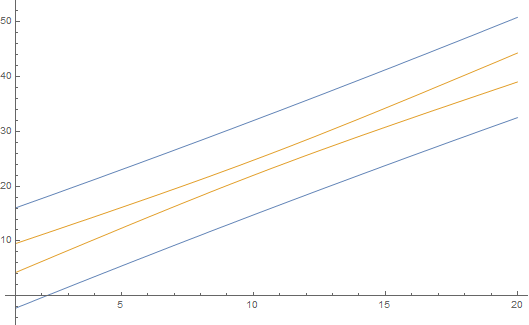
\includegraphics[width=0.5\textwidth]{imagenes1/bandas.png}
\end{figure}

\section{Diagnosis de las hipótesis del modelo. Análisis de residuos. Observaciones atípicas e influyentes}

\subsubsection{Lienalidad}
Recordemos que la hipótesis de linealidad era la siguiente
\begin{align*}
    E(u_i) = 0 \Longleftrightarrow E(y_i | x_i) = \beta_0 + \beta_1 x_i, \quad \forall i = 1, \dots n.
\end{align*}
Para ver gráficamente si se cumple esta hipótesis, podemos representar la gráfica de $e_i$ frente a $x_i$, o bien la gráfica de $e_i$ frente de $\widehat{y}_i$. Si dichas gráficas no presentan una estructura funcional, entonces podemos decir que se cumple la hipótesis de linealidad. Podemos ver que esta hipótesis se cumple en las siguientes gráficas
\begin{figure}[H]
    \begin{subfigure}[b]{0.45\textwidth}
        \centering
        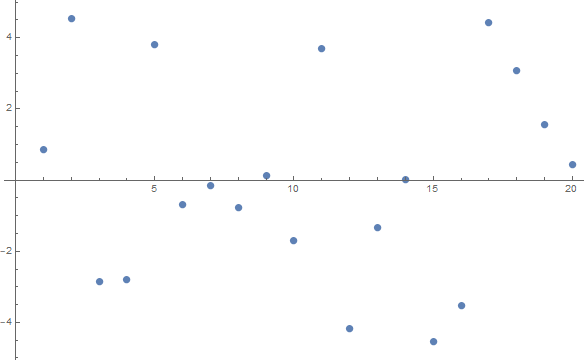
\includegraphics[width=0.45\textwidth]{imagenes1/linealidadx.png}
        \caption{Gráfica de $e_i$ frente a $x_i$.}
    \end{subfigure}
    \begin{subfigure}[b]{0.45\textwidth}
        \centering
        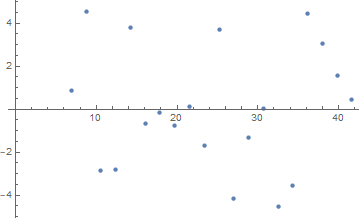
\includegraphics[width=0.45\textwidth]{imagenes1/linealidady.png}
        \caption{Gráfica de $e_i$ frente a $\widehat{y}_i$.}
    \end{subfigure}
\end{figure}
De no cumplirse la hipótesis de linealidad, podríamos tratar de aplicar alguna transformación a $X$.
\subsubsection{Homocedasticidad}
Recordemos que la hipótesis de homocedasticidad es la siguiente
\begin{align*}
    Var(u_i) = \sigma^2 \Longleftrightarrow Var(y_i | x_i) = \sigma^2, \quad \forall i = 1, \dots n.
\end{align*}
Para ver gráficamente si se cumple esta hipótesis, podemos representar la gráfica de $e_i$ frente a $\widehat{y}_i$. Si dicha gráfica está acotada por ''rectas'' paralelas, entonces podemos decir que si se cumple la hipótesis de homocedasticidad. Podemos ver que esta hipótesis se cumple en la siguiente gráfica
\begin{figure}[H]
    \centering
    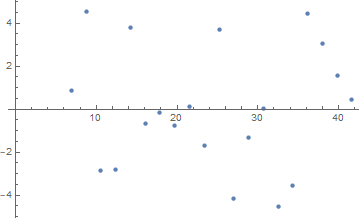
\includegraphics[width=0.35\textwidth]{imagenes1/linealidady.png}
\end{figure}

De no cumplirse la hipótesis de linealidad, podriamos tratar de aplicar alguna transformación a $Y$.

\subsubsection{Normalidad}
Podemos hacer lo siguiente
\begin{enumerate}
    \item[a)] Gráficos descriptivos: Histograma de los residuos o diagrama de caja y bigotes.
          \begin{figure}[H]
              \centering
              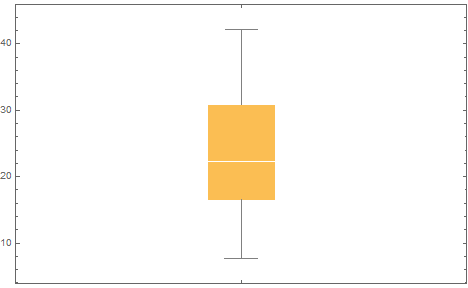
\includegraphics[width=0.35\textwidth]{imagenes1/histo.png}
          \end{figure}
    \item[b)] Gráficos de probabilidad normal.
          \begin{itemize}
              \item $P-P$: Probabilidad de datos frente a lo normal.
              \item $Q-Q$: Cuantiles de los datos frente a la normal.
          \end{itemize}
          \begin{figure}[H]
              \centering
              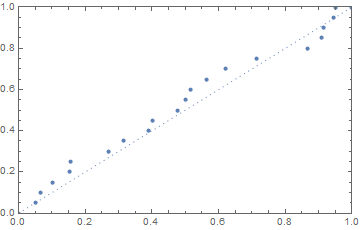
\includegraphics[width=0.35\textwidth]{imagenes1/probdatos.png}
          \end{figure}
    \item[c)] Graficar los residuos frente a $x_i$ o frente a $\widehat{y}_i$.
\end{enumerate}

\subsubsection{Observaciones atípicas}
Una observación atípica es un valor que es numéricamente distinto al resto de los datos. Visualmente, es un dato que se sale del patrón.
Las observaciones atípicas pueden ser indicativas de errores de observación o errores en el modelo. Un error de observación se debe a datos que pertenecen a una población diferente del resto de muestras, mientras que un error en el modelo puede ser debido a que la muestra depende una variable desconocida que no se han tenido en cuenta.

\subsubsection{Observaciones influyentes}
Una observación influyente $(x_A, y_A)$ es una observación atípica cuya exclusión produce un cambio drástico en la recta de regresión. Puede ser causada por un error de observación o por un modelo incorrecto. Algunas posibles causas de que el modelo sea incorrecto son:
\begin{itemize}
    \item La relación entre $x$ e $y$ no es lineal cerca de $x_A$.
    \item La varianza aumenta mucho con $x$.
    \item Una variable desconocida ha tomado un valor distinto en $x_A$.
\end{itemize}

\subsubsection{Puntos palanca}
Los puntos palanca son observaciones con un valor alto de $p_i$.
Estos tienen la capacidad de alterar en gran medida la recta de regresión.

\section{Transformaciones}
Cuando el diagrama de dispersión entre las dos variables o el de los residuos presenta indicios de incumplimiento de alguna hipótesis básica, entonces hay que abandonar el modelo inicial por uno menos simple o bien aplicar alguna transformación a los datos.
